\documentclass{article}
\usepackage{amsmath}
\usepackage{amsthm}
\usepackage{amsfonts}
\usepackage{amssymb}
\usepackage{bbold}
\usepackage{dsfont}
\usepackage{graphicx}
\usepackage{cleveref}
\usepackage{bm}
\usepackage{booktabs}
\usepackage{siunitx}
\usepackage{xcolor}
\usepackage{pdfpages}
\usepackage[utf8]{inputenc}
\usepackage[english]{babel}
\newtheorem{definition}{Definition}
\newtheorem{example}{Example}
\newcommand{\exP}[1]{\mathrm{e}^{#1}}
\newcommand{\dif}{\mathrm{d}}
\renewcommand{\vec}[1]{\mathbf{#1}}
\newcommand{\pdagger}{{\phantom{\dagger}}}
\newcommand{\state}[1]{\vert #1\rangle}
\newcommand{\cstate}[1]{\langle #1\vert}
\newcommand{\tr}[1]{\mathrm{tr}\left\{#1\right\}}
\newcommand{\trs}[2]{\, \mathrm{tr}_{#1}\{#2\}}
\newcommand{\expc}[3]{\langle #1\vert #2 \vert #3\rangle}
\usepackage[doi=false,url=false,isbn=false,backend=bibtex,style=nature,natbib=true,sorting=none]{biblatex}
\bibliography{bib.bib}
\usepackage{geometry}
\geometry{
	a4paper,
	total={170mm,257mm},
	left=15mm,
	right=15mm,
	top=15mm,
}
\begin{document}
\title{Report 28: Alternative ordering of environment indices}
\maketitle
\section{Parameters}
\begin{itemize}
	\item $N=2$ and $N=3$ sites
	\item $\varepsilon_0 = -\SI{240}{\milli\electronvolt}$
	\item $\omega_0 = \SI{100}{\milli\electronvolt}$
	\item $t_0=\SI{40}{\milli\electronvolt}$
	\item $\lambda_0=\SI{1}{\milli\electronvolt}$
	\item $\lambda_1=\SI{0.1}{\milli\electronvolt}$
	\item $\Gamma_0=\SI{10}{\milli\electronvolt}$
	\item $k_B T=\SI{25}{\milli\electronvolt}$
	\item $t_1=0.2t_0=\SI{8}{\milli\electronvolt}$
	\item $V=\SI{0.5}{\volt}$
	\item $N_p=12$.
\end{itemize}
\section{Order of environment indices}
The order of the environment indices that has been previously employed and the new ordering are represented schematically in the figure below. The previous ordering (called v1 in the following) is $(s,\ell,p,\sigma)$, where $s=\uparrow,\downarrow$ is the spin, $\ell=L,R$ the lead, $p=1\dots N_p$ the Pad\'{e} pole and $\sigma=+,-$ the electron/hole index. The new ordering (v2) is $(s,p,\ll,\sigma)$ and places core tensors of the different leads closer to each other.
\begin{figure}[!h]
	\centering
	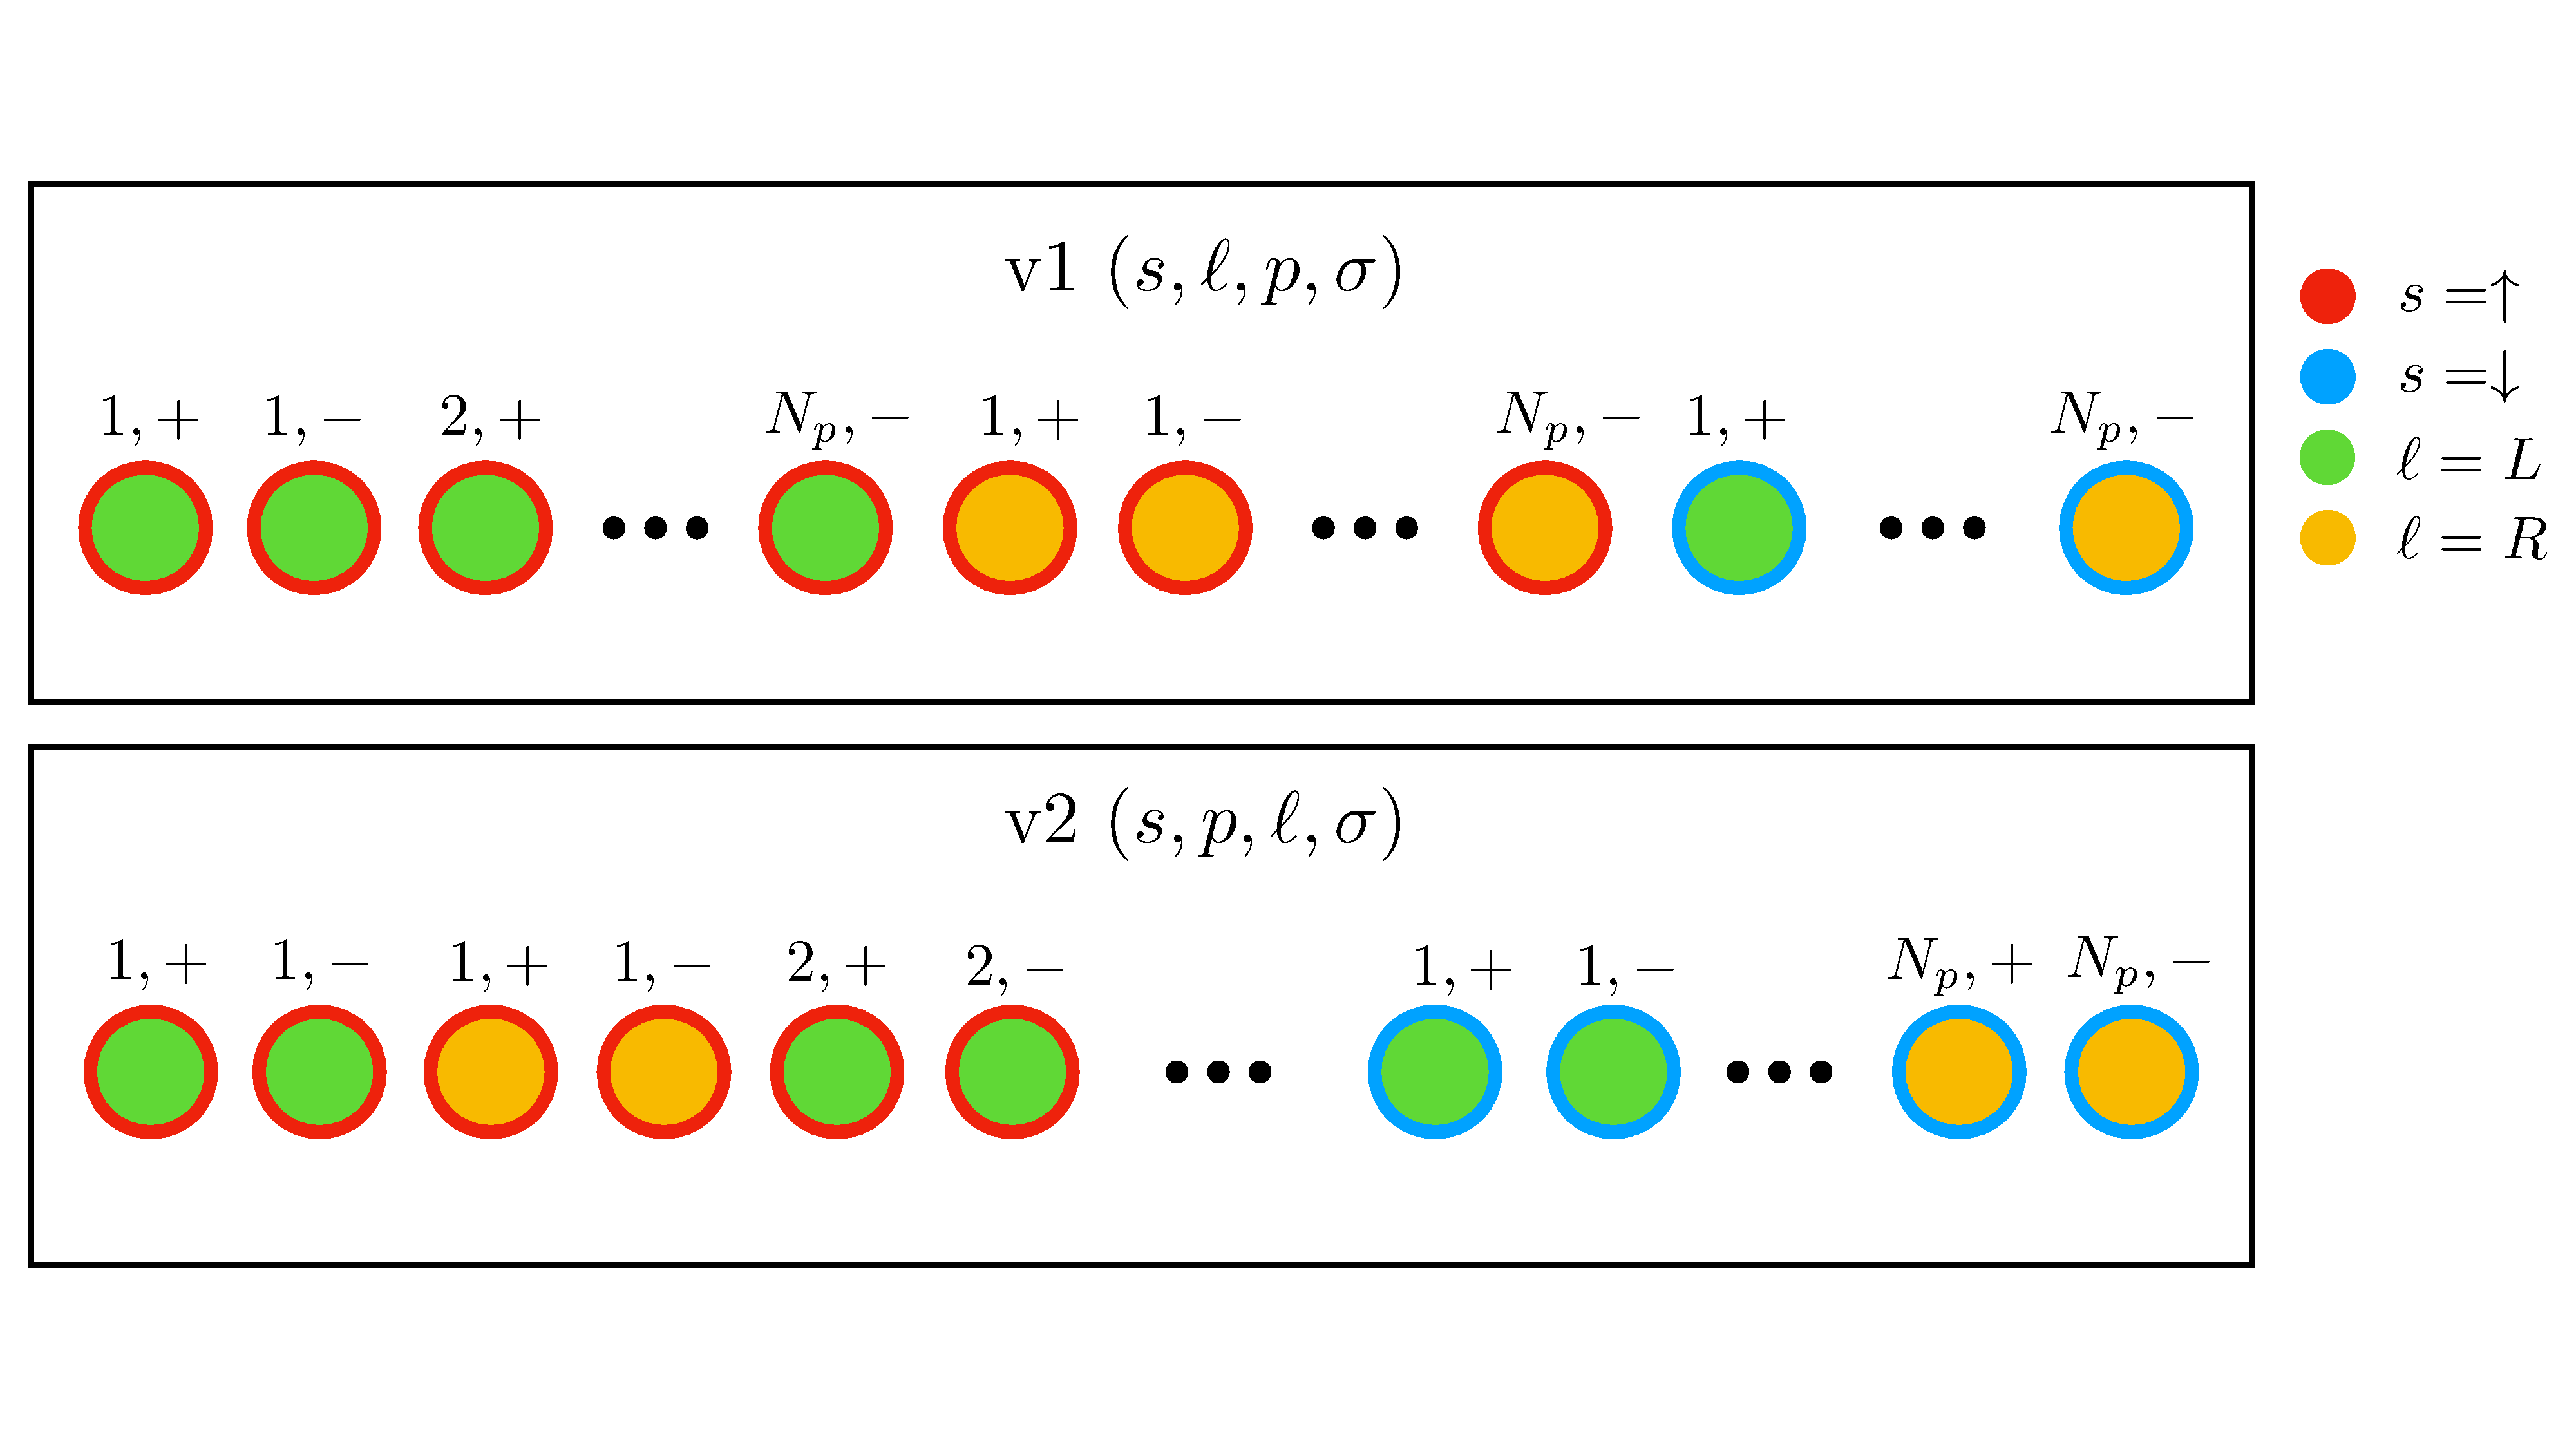
\includegraphics[width=0.8\textwidth]{figs/scheme.pdf}
\end{figure}
\section{Overview of results}
\begin{itemize}
	\item \Cref{sec:1}: Test of implementation for a two-site system
	\item \Cref{sec:2}: Comparison of both ordering schemes for a three-site system
\end{itemize}
\section{$N=2$}\label{sec:1}
The molecule is represented by four electronic states and one vibrational mode. This system acts as a test of the implementation. \Cref{fig:1} shows the charge current and the average rank for two cases: $t_1=\SI{0}{\milli\electronvolt}$ and $t_1=\SI{8}{\milli\electronvolt}$. No significant change of the new ordering is observed in this system, both without and with electron-vibrational coupling.
\begin{figure}[!h]
	\centering
	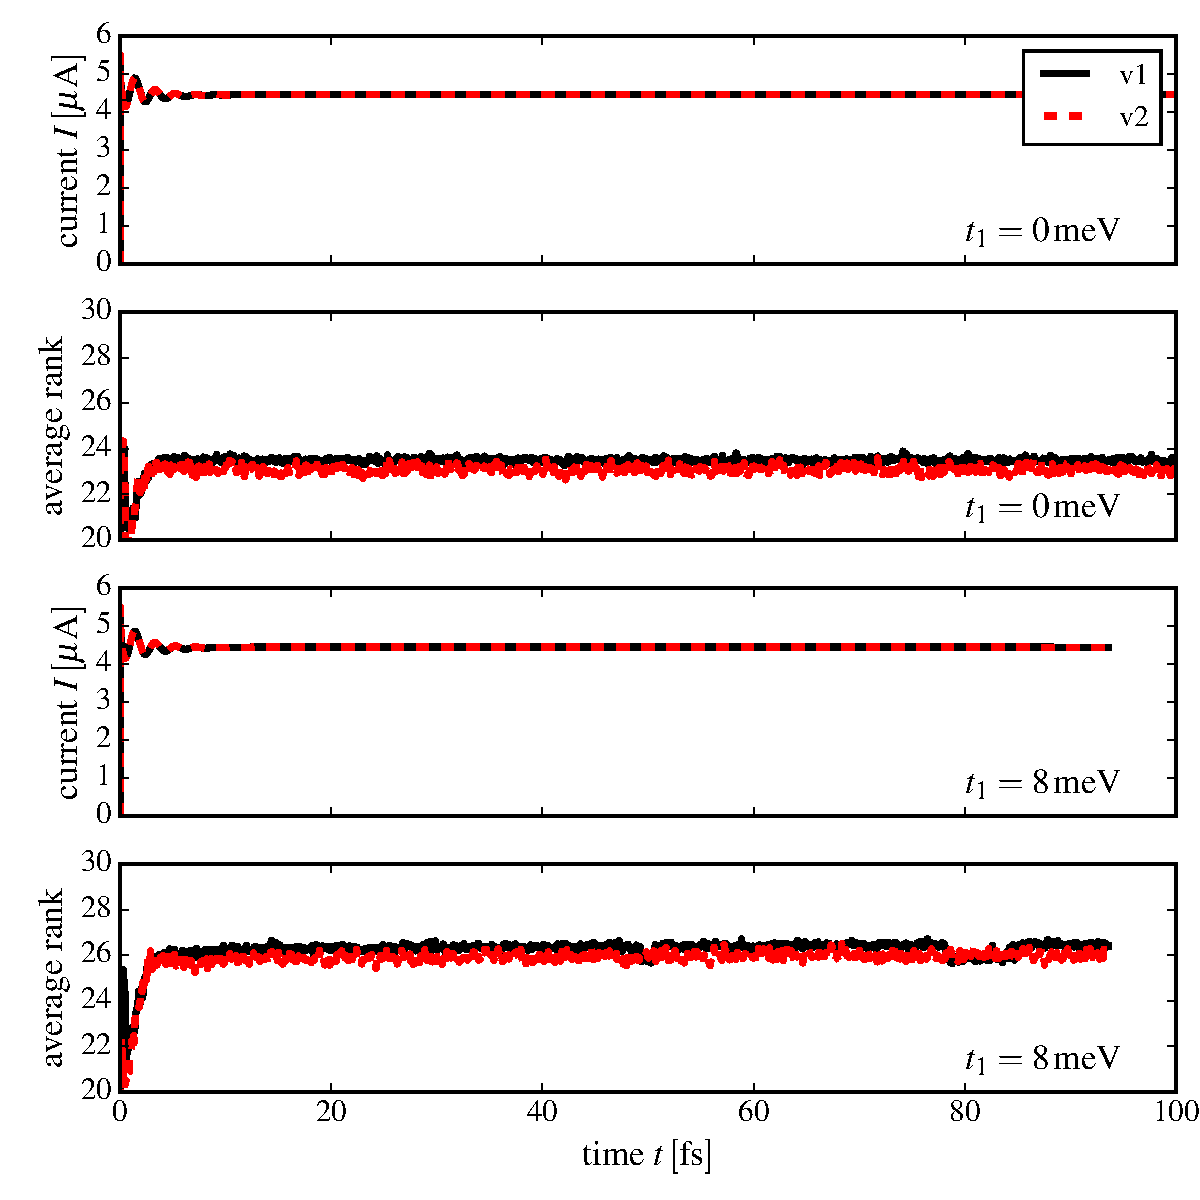
\includegraphics[width=0.7\textwidth]{figs/L1x2_tamen_alt_ordering_res.pdf}
	\caption{$n_\mathrm{vib}=10$ and $\mathrm{tol}=10^{-3}$}\label{fig:1}
\end{figure}
\clearpage
\section{$N=3$}\label{sec:2}
The system size is consisting of six electronic states and two vibrational modes. The electron-vibrational coupling here is $t_1=\SI{8}{\milli\electronvolt}$. \Cref{fig:2} shows the charge current, average rank, and maximal rank for the two orderings. The average rank of the new ordering is approximately 20\% larger than of the previous ordering. The maximal rank, however, is for both orderings the same. This suggests, that the bottleneck of the rank is not related to the ordering of the reservoir indices, but rather to correlation between electronic and vibrational dof in the molecule. This statement is supported by a large rank predominantly between electronic of the molecule, shown in \cref{fig:3}. Herein, the top figure is for v1 and the bottom figure for the v2 ordering. Here, the horizontal axis is the bond number, with bond numbers 1 to 79 corresponding to bonds between reservoir indices.   
\begin{figure}[!h]
	\centering
	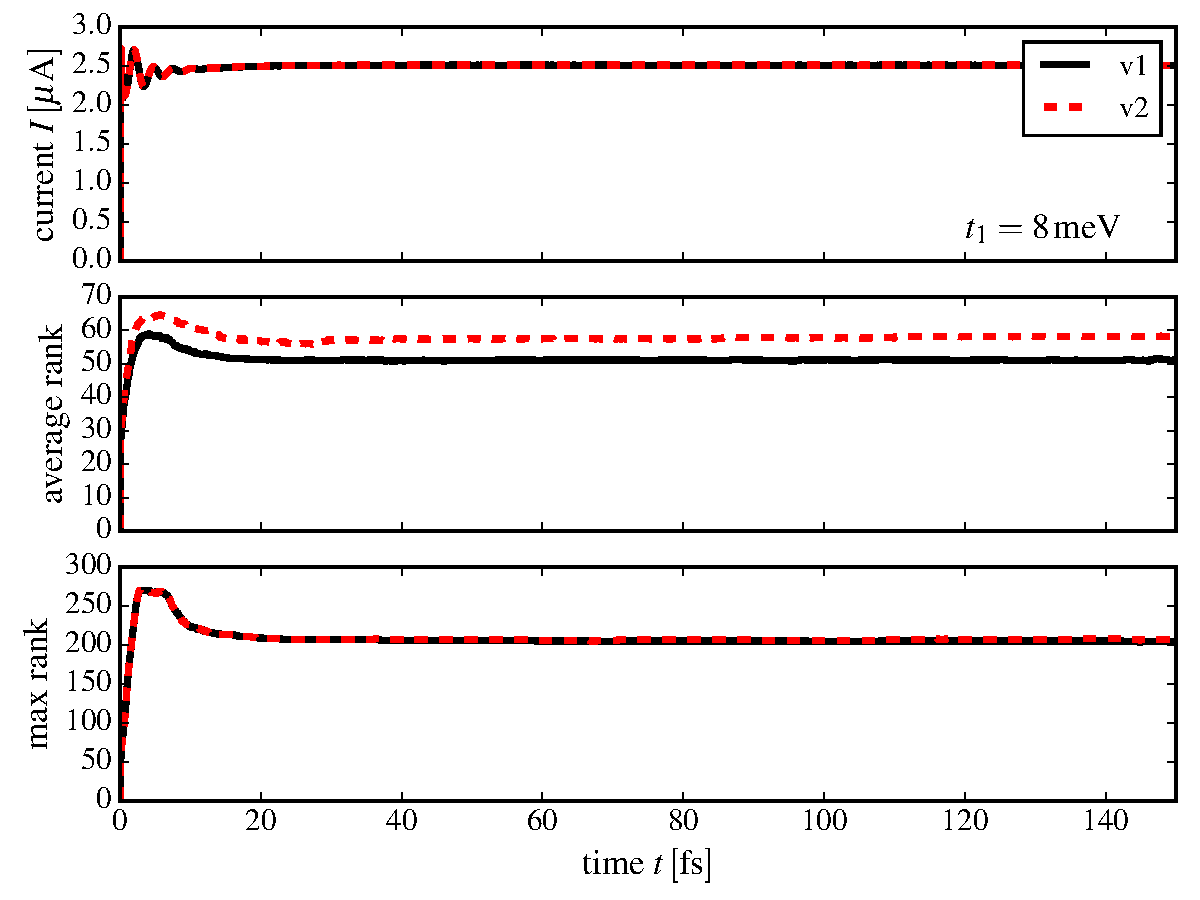
\includegraphics[width=0.7\textwidth]{figs/L1x3_t1_2_tamen_alt_ordering_res.pdf}
	\caption{$n_\mathrm{vib}=10$ and $\mathrm{tol}=10^{-3}$}\label{fig:2}
\end{figure}
\begin{figure}[!h]
	\centering
	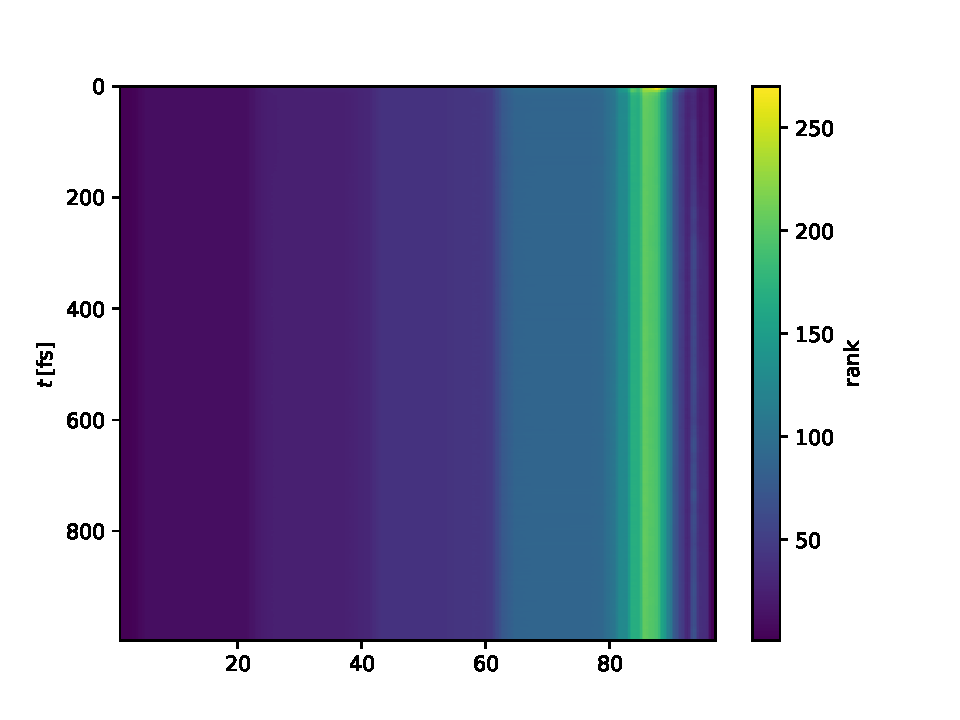
\includegraphics[width=0.6\textwidth]{figs/L1x3_t1_2_P_V10_nvib10_tol1e-3_rank.pdf}
	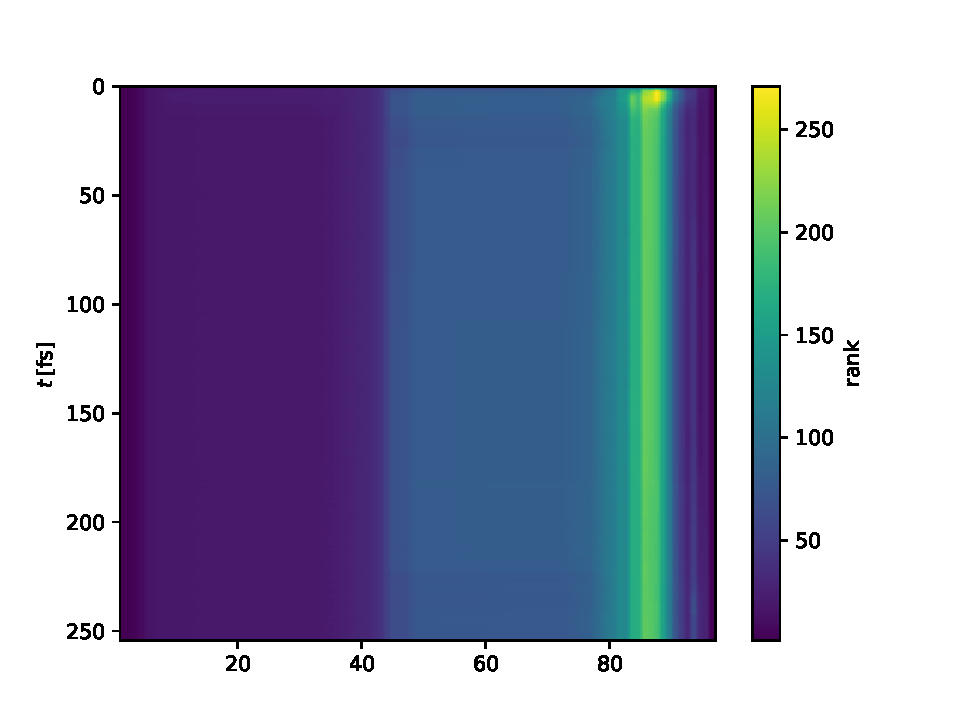
\includegraphics[width=0.6\textwidth]{figs/L1x3_t1_2_P_V10_nvib10_tol1e-3_rank_v2.pdf}
	\caption{Time dependent rank distribution in the TT for $n_\mathrm{vib}=10$ and $\mathrm{tol}=10^{-3}$. Top: v1, bottom: v2}\label{fig:3}
\end{figure}
 


\end{document}


